\newcommand\COURSE{ciss445}
\newcommand\ASSESSMENT{t01}
\newcommand\ASSESSMENTTYPE{Test}
\newcommand\POINTS{\textwhite{xxx/xxx}}

\makeatletter
\DeclareOldFontCommand{\rm}{\normalfont\rmfamily}{\mathrm}
\DeclareOldFontCommand{\sf}{\normalfont\sffamily}{\mathsf}
\DeclareOldFontCommand{\tt}{\normalfont\ttfamily}{\mathtt}
\DeclareOldFontCommand{\bf}{\normalfont\bfseries}{\mathbf}
\DeclareOldFontCommand{\it}{\normalfont\itshape}{\mathit}
\DeclareOldFontCommand{\sl}{\normalfont\slshape}{\@nomath\sl}
\DeclareOldFontCommand{\sc}{\normalfont\scshape}{\@nomath\sc}
\makeatother

\input{myquizpreamble}
\input{yliow}
\input{\COURSE}
\textwidth=6in

\renewcommand\TITLE{\ASSESSMENTTYPE \ \ASSESSMENT}

\newcommand\topmattertwo{
\topmatter
\score \\ \\
Open \texttt{main.tex} and enter answers (look for
\texttt{answercode}, \texttt{answerbox}, \texttt{answerlong}).
Turn the page for detailed instructions.
To rebuild and view pdf, in bash shell execute \texttt{make}.
To build a gzip-tar file, in bash shell execute \texttt{make s} and
you'll get \texttt{submit.tar.gz}.
}

\newcommand\tf{T or F or M}
\newcommand\answerbox[1]{\textbox{#1}}
\newcommand\codebox[1]{\begin{console}#1\end{console}}

\usepackage{pifont}
\newcommand{\cmark}{\textred{\ding{51}}}
\newcommand{\xmark}{\textred{\ding{55}}}

\newcounter{qc}
\newcommand\nextq{
%\newpage
\addtocounter{qc}{1}
Q{\theqc}.
}

\DefineVerbatimEnvironment%
 {answercode}{Verbatim}
 {frame=single,fontsize=\footnotesize}

\newenvironment{largebox}[1]{%
 \boxparone{#1}
}
{}

\usepackage{environ}
\let\oldquote=\quote
\let\endoldquote=\endquote
\let\quote\relax
\let\endquote\relax

% ADDED 2021/09/09
\renewcommand\boxpar[1]{
 \[
  \framebox[\textwidth][c] {
   \parbox[]{\dimexpr\textwidth - 0.25cm} {#1}
  }
 \]
}

\NewEnviron{answerlong}%
  {\vspace{-1mm} \global\let\tmp\BODY\aftergroup\doboxpar}

\newcommand\doboxpar{%
  \let\quote=\oldquote
  \let\endquote=\endoldquote
  \boxpar{\tmp}
}

\newenvironment{mcq}[7]%
{% begin code
#1 \dotfill{#2}
 \begin{tightlist}
 \item[(A)] #3
 \item[(B)] #4
 \item[(C)] #5
 \item[(D)] #6
 \item[(E)] #7 
 \end{tightlist}
}%
{% end code
} 

\renewcommand\EMAIL{}
\newcommand\score{%
\vspace{-0.6in}
\begin{flushright}
Score: \answerbox{\POINTS}
\end{flushright}
\vspace{-0.4in}
\hspace{0.7in}\AUTHOR
\vspace{0.2in}
}

\newcommand\blankline{\mbox{}\\ }

\newcommand\ANSWER{\textsc{Answer: }}

\newcommand\LATEXHELPTHREEFIVEZERO{
In the \texttt{answerlong}, you will need to enter \LaTeX\ code for
mathematical notation.
Some incomplete or wrong answers are included in the \texttt{answerlong}
so that all you need to do is to make minor modifications.
Note that \texttt{answercode} is for writing code/pseudocode and
does not require mathematical notation.

Here are some pointers on writing math \LaTeX\ code:
\begin{enumerate}[nosep]

\item For \lq\lq inline math mode", use \texttt{\$...\$}.
Example: \texttt{\$x\ =\ 42\ +\ y\$} gives you $x = 42 + y$.
(Mathematical expressions have their own spacing, special symbols,
and are in italics.)

\item For \lq\lq display math mode", use \texttt{\textbackslash[...\textbackslash]}.
Example: \texttt{\textbackslash[\ x\ =\ 42 \textbackslash]} gives you \[ x = 42 \]
(Display math mode is used for emphasis.)

\item Here's how you do fractions:
\texttt{\$\textbackslash frac\{1\}\{2\}\$} gives you $\frac{1}{2}$.

\item Here's how you do subscript:
\texttt{\$t\_\{123\}\$} gives you $t_{123}$. 

\item Here's how you do superscript:
\texttt{\$n\^{}\{123\}\$} gives you $n^{123}$.
\end{enumerate}

The above information should be enough for this quiz.
For more information on \LaTeX\, you can go to
\href{http://bit.ly/yliow0/}{my website},
click on Yes you are one of my students, scroll down to the Tutorials
section and click on latex.pdf.
}

\newcommand\LATEXHELPTHREEFIVEZEROB{
In the \texttt{answerlong}, you will need to enter \LaTeX\ code for
mathematical notation.
Some incomplete or wrong answers are included in the \texttt{answerlong}
so that all you need to do is to make minor modifications.
Note that \texttt{answercode} is for writing code/pseudocode and
does not require mathematical notation.

Here are some pointers on writing math \LaTeX\ code:
\begin{enumerate}[nosep]

\item For \lq\lq inline math mode", use \texttt{\$...\$}.
Example: \texttt{\$x\ =\ 42\ +\ y\$} gives you $x = 42 + y$.
(Mathematical expressions have their own spacing, special symbols,
and are in italics.)

\item For \lq\lq display math mode", use \texttt{\textbackslash[...\textbackslash]}.
Example: \texttt{\textbackslash[\ x\ =\ 42 \textbackslash]} gives you \[ x = 42 \]
(Display math mode is used for emphasis.)

\item Here's how you do fractions:
\texttt{\$\textbackslash frac\{1\}\{2\}\$} gives you $\frac{1}{2}$.

\item Here's how you do subscript:
\texttt{\$t\_\{123\}\$} gives you $t_{123}$. 

\item Here's how you do superscript:
  \texttt{\$n\^{}\{123\}\$} gives you $n^{123}$.
  
\item Here's how you do log:
  \texttt{\$\textbackslash lg n\$} gives you $\lg n$.
\end{enumerate}

The above information should be enough for this quiz.
For more information on \LaTeX\, you can go to
\href{http://bit.ly/yliow0/}{my website},
click on Yes you are one of my students, scroll down to the Tutorials
section and click on latex.pdf.
}



\renewcommand\AUTHOR{Carl Dalebout} % CHANGE TO YOURS

\begin{document}
\topmattertwo

\begin{enumerate}

\li This is a closed-book, no-calculator, no-computer, no-discussion test.

\li Your solution must be written in the box provided. Anything outside the box
is not considered part of the solution.
Everything inside the box IS considered part of the solution.

\li Do NOT provide multiple solutions. If you do, I get to pick ONE to grade.
(I'm very good at picking solution -- the wrong one).

\li Write neatly. If I cannot read your solution easily you will get zero.

\li
For the OCAML coding problems,
your grade will be based on passing a lists of tests cases.
If your code passes all the test cases,
you get all the points for that question;
if it does not pass any test cases you will get 0.
Not all test cases are shown below.
For some questions, test cases are not shown.

\li 
Cheating is a serious academic offense. If caught you will receive an
immediate score
of -100\%.

\end{enumerate}

\newpage
\begin{python}
from latextool_basic import *
test_score_table()
\end{python}



\newpage
\nextq
The following are the phases in source code compilation:

\begin{center}
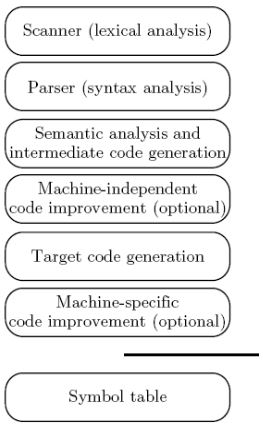
\includegraphics[width=2.5in]{pic.JPG}
\end{center}

(a) What is the input for the scanner phase?
\\
\ANSWER
\begin{answercode}

\end{answercode}

(b) What is the output during the scanner phase?
\\
\ANSWER
\begin{answercode}

\end{answercode}

(c) What is the input for the parser phase?
\\
\ANSWER
\begin{answercode}
  
\end{answercode}

(d) What is the output during the parser phase?
\\
\ANSWER
\begin{answercode}

\end{answercode}

%===============================================================================
\newpage
\nextq
Write a function \verb!quadratic! such that
\verb!(quadratic a b c)! returns a function that computes the $y$-value
of the quadratic equation $y = ax^2 + bx + c$.
For instance 

\begin{console}[frame=none]
        Test                       Expected value
        (quadratic 0 1 2) 5        0 * 5 * 5 + 1 * 5 + 2
        (quadratic 1 2 3) 3        1 * 3 * 3 + 2 * 3 + 3
        (quadratic 2 3 4) 7        2 * 7 * 7 + 3 * 7 + 4
\end{console}

\ANSWER
\begin{answercode}
  
	let quadratic = fun a -> fun b -> fun c -> fun x ->
		a * x * x + b * x + c
	;;

\end{answercode}

%===============================================================================
\newpage
\nextq
Write a \verb!second! function such that \verb!second xs!
returns a list that contains exactly the second value of
the list \verb!xs!.
If \verb!xs! does not have at least two values, \verb![]! is returned.

\begin{console}[frame=none]
	Test                         Expected value
	second []                    []
    second [42]                  []
	second [2;9]                 [9]
	second [3;4;5]               [4]
    second [1.1; 2.2; 3.3; 4.4]  [2.2]
\end{console}

\ANSWER
\begin{answercode}
  let second = fun x -> 
  match x with 
  | [] -> []
  | x::xs -> 
	match xs with 
	| [] -> []
	| y::ys -> y
  ;;
\end{answercode}

%===============================================================================
\newpage
\nextq
What is the value of the \verb!x! in the following binding:
\begin{console}
let x = (fun f -> (fun x -> f(f x))) (fun x -> x * x) 2;;
\end{console}
or write ERROR.

\ANSWER
\begin{answercode}
 (int -> int) -> int -> (int -> ((int -> int ) -> int)) -> int 
\end{answercode}

%===============================================================================
\newpage
\nextq
Write down the type for each of the following expressions.
Write ERROR if there's an error in the expression.
\begin{tightlist}
\li Recall that the type of a function look like
\verb!'a -> 'b!.    
For instance the type of \verb!fun x -> x + 1! is
\verb!int -> int! and the type of
\verb!fun x -> fun y -> x + y! is \verb!int -> int -> int!
and the type of
\verb!fun x -> fun y -> (x < y)! is \verb!'a -> 'a -> bool!.
\li The type of a list looks like \verb!'a list!.
For instance the type of \verb![1;2;3]! is
\verb!int list!.
\li The type of a 2-tuple looks like \verb!'a * 'b!.
For instance the type of \verb!(1, 2.4)! is
\verb!int * float!.
The type for 3-tuple, 4-tuple, etc. are analgous.
\li If you use type parameters, make sure you use \verb!'a!,
\verb!'b!, \verb!'c!, etc. in that order.
\end{tightlist}


(a) \verb!if 1 = 2 then [3] else [4]!
\\
\ANSWER
\begin{answercode}
int -> int -> bool -> int
\end{answercode}

(b) \verb!fun x -> fun y -> y::x::[1]!
\\
\ANSWER
\begin{answercode}
int -> int -> int list
\end{answercode}

(c) \verb!fun x -> fun y -> y::[x]!
\\
\ANSWER
\begin{answercode}
'a -> 'a -> list 'a
\end{answercode}

(d) \verb!fun x -> fun y -> (y (x + 1) +. 3.0)!
\\
\ANSWER
\begin{answercode}
Error addition between and int and a float
\end{answercode}

(e) \verb!fun x -> fun y -> y x!
\\
\ANSWER
\begin{answercode}
Error Two Outputs
\end{answercode}

(f) \verb!fun x -> fun y -> x y!
\\
\ANSWER
\begin{answercode}
	Error Two Outputs
\end{answercode}

%===============================================================================
\newpage
\nextq
Write a number guessing game. Call \verb!(guess 42)!
and the user is prompted to enter a guess. If the number
entered is 42, the program will stop. If the number entered is
$<$ 42, the program will ask the user to try a larger number. If
the number entered is $>$ 42, the program will ask the user to
try a smaller number.

To get an integer value from the user do this:
\begin{console}
let x = read_int ();;
\end{console}

Here's a sample execute:
{\small
\begin{console}[commandchars=\\\{\}]
utop # guess 42;;
guess my int: \userinput{1}
try higher ...
guess my int: \userinput{100}
try lower ...
guess my int: \userinput{50}
try lower ...
guess my int: \userinput{25}
try higher ...
guess my int: \userinput{30}
try higher ...
guess my int: \userinput{40}
try higher ...
guess my int: \userinput{45}
try lower ...
guess my int: \userinput{43}
try lower ...
guess my int: \userinput{42}
correct!!!
- : unit = ()
\end{console}
}

Turn page ...
\newpage
\ANSWER
\begin{answercode}
let guess = fun value ->
	let x = read_int() in
	if x = value then
		correct!!!
	else if x > value then
		"try lower ..."
	else 
		"try higher ..."
;;	
\end{answercode}

%===============================================================================
\newpage
\nextq
Write a function \verb!reverse_at! so that \verb!(reverse_at list n)!
returns the element of the list at index \verb!n! in the reverse order,
i.e., index 0 means the last value, index 1 means the second last value, etc.
Ignore the case where \verb!n < 0! or \verb!n >=! the size of the list.

\begin{Verbatim}
	Test                       Expected values
	reverse_at [5;3;1] 0       1
	reverse_at [2;4;6] 1       4
	reverse_at [1;3;5;7] 3     1
\end{Verbatim}


\ANSWER
\begin{answercode}
	let reverse_at = fun list -> fun n ->
		//need to come back to this 
\end{answercode}

%===============================================================================
\newpage
\nextq
Write a function \verb!rev! that reverses a list.
For instance after
\verb!(rev [1; 3; 5])!
is \verb![5; 3; 1]!.
Any recursion used must be tail recursion.
In other words,
\verb!(rev list)!
should call another function that returns the reverse of \verb!list!
and this function computes the reverse of
\verb!list! using tail recursion.

\ANSWER
\begin{answercode}
	let rec rev = fun list -> fun accum
	match list with
	| [] -> accum
	| x::xs -> rev xs x@accum
	;;
\end{answercode}

%===============================================================================
\newpage
\nextq
Write a function \verb!seteq! that compares two lists are the same,
treating them as sets.
For instance
\verb!seteq [1;3;5] [5;3;3;1;1;3]!
is true.
In other words
\verb!seteq xs ys! is true exactly when the values in \verb!xs!
are in \verb!ys! and the values in \verb!ys! are in \verb!xs!.
You need not use tail recursion.
\\
\ANSWER
\begin{answercode}
	let rec seteq = fun list1 -> fun list2 ->
		match list1 with
		| [] -> true
		| x::xs -> 
			let rec loop = fun value -> list ->
				match list with 
				| [] -> false
				| y::ys -> if y = value then
							true
						   else
						   	loop value ys
							in
			if (loop x list2) then
				seteq xs list2
			else
				false
	;;
\end{answercode}

%===============================================================================
\newpage
\nextq
Write a function \verb!powerset! that computes the powerset
of a list.
For instance after
\begin{console}
let xs = powerset [1;3;5];;
\end{console}
\verb!xs! is \verb![[]; [1]; [3]; [5]; [1;3]; [1;5]; [3;5]; [1;3;5]]!.
The lists need not appear in the above order.
The values in a list of the above list need not be in the above order --
for instance \verb![1;3]! can be \verb![3;1]!.
In other words, you can view each list as a set.

\ANSWER
\begin{answercode}
% powerset [1] = [[1]; []]
% powerset [1; 2] = [[1]; [2]; [1; 2]; []]
% powerset [1; 2; 3] = [[1]; [2]; [3]; [1; 2]; [1; 3]; [2; 3]; [1; 2; 3]; []]

let rec powerset = fun list ->
match list with 
| [] -> [[]]
| x -> x::[]
| x::xs -> x::(powerset xs)::list::[]


\end{answercode}


%===============================================================================
\newpage
\nextq
You are given this binary tree:
\begin{console}
type 'a bintree = Empty
                | Node of ('a * 'a bintree * 'a bintree)
;;
\end{console}
(a) Write a function \verb!has_element! such that
\verb!has_element t v! is true iff the value \verb!v! is in the
tree \verb!t!.
For instance
\begin{console}
utop # let t = Node (5, Node (6, Empty, Empty), Node (1, Empty, Empty));;
val t : int bintree = Node (5, Node (6, Empty, Empty), Node (1, Empty, Empty))
utop # has_element t 5;;
- : bool = true
utop # has_element t 7;;
- : bool = false
\end{console}
\ANSWER
\begin{answercode}
let rec has_element = fun t -> fun v ->
	match t with 
	| Empty -> false
	| (x * Left * Right) -> if x = v then 
								true
					 		else
								if(has_element Left v) then
									true
								else if (has_element Right v) then
									true
								else
									false
;;
									
\end{answercode}

(b)
Write a function \verb!subtree! such that 
\verb!subtree t v! is the subtree of \verb!t! with \verb!v! as root.
For instance
\begin{console}
utop # let t = Node (5, Node (6, Empty, Empty), Node (1, Empty, Empty));;
val t : int bintree = Node (5, Node (6, Empty, Empty), Node (1, Empty, Empty))
utop # subtree t 5;;
- : int bintree = Node (5, Node (6, Empty, Empty), Node (1, Empty, Empty))
utop # subtree t 6;;
- : int bintree = Node (6, Empty, Empty)
utop # subtree t 1;;
- : int bintree = Node (1, Empty, Empty)
utop # subtree t 0;;
- : int bintree = Empty
\end{console}
(You can assume that the values in the tree are unique.)
\\
\ANSWER
\begin{answercode}
let rec subtree = fun t -> fun v ->
	match t with
	| Empty -> Empty
	| (x * Left * Right) -> if x = v then 
								t
							else if (subtree Left v = Empty) then
								if(subtree Right v = Empty) then
									Empty
								else 
								 	Empty
;;

\end{answercode}


%------------------------------------------------------------------------------
%\newpage
%
\textsc{Instructions}

In \verb!main.tex! change the email address in
\begin{console}
\renewcommand\AUTHOR{jdoe5@cougars.ccis.edu} 
\end{console}
yours.
In the bash shell, execute \lq\lq \verb!make!" to recompile \verb!main.pdf!.
Execute \lq\lq \verb!make v!" to view \verb!main.pdf!.
Execute \lq\lq \verb!make s!" to create \verb!submit.tar.gz! for submission.

For each question, you'll see boxes for you to fill.
You write your answers in \verb!main.tex! file.
For small boxes, if you see
\begin{console}[frame=single=single,fontsize=\small]
1 + 1 = \answerbox{}.
\end{console}
you do this:
\begin{console}[frame=single=single,fontsize=\small]
1 + 1 = \answerbox{2}.
\end{console}
\verb!answerbox! will also appear in
\lq\lq true/false" and \lq\lq multiple-choice"
questions.

For longer answers that needs typewriter font, if you see
\begin{console}[frame=single=single, fontsize=\small]
Write a C++ statement that declares an integer variable name x.
\begin{answercode}
\end{answercode}
\end{console}
you do this:
\begin{console}[frame=single=single, fontsize=\small]
Write a C++ statement that declares an integer variable name x.
\begin{answercode}
int x;
\end{answercode}
\end{console}
\verb!answercode! will appear in questions asking for
code, algorithm, and program output.
In this case, indentation and spacing is significant.
For program output, I do look at spaces and newlines.

For long answers (not in typewriter font) if you see
\begin{console}[frame=single=single, fontsize=\small]
What is the color of the sky?
\begin{answerlong}
\end{answerlong}
\end{console}
you can write
\begin{console}[frame=single=single, fontsize=\small]
What is the color of the sky?
\begin{answerlong}
The color of the sky is blue.
\end{answerlong}
\end{console}
For students beyond 245: You can put \LaTeX\ commands in
\verb!answerbox! and 
\verb!answerlong!.

A question that begins with \lq\lq T or F or M"
requires you to identify whether it is true or
false, or meaningless.
\lq\lq Meaningless" means something's wrong with the statement and
it is not well-defined.
Something like \lq\lq $1 +_2$" or \lq\lq $\{2\}^{\{3\}}$" is not
well-defined.
Therefore a question such as
\lq\lq Is $42 = 1 +_2$ true or false?" or
\lq\lq Is $42 = \{2\}^{\{3\}}$ true or false?"
does not make sense.
\lq\lq Is $P(42) = \{42\}$ true or false?" is meaningless because $P(X)$
is only defined if $X$ is a set.
For \lq\lq Is 1 + 2 + 3 true or false?", \lq\lq 1 + 2 + 3" is well--defined but
as a
\lq\lq numerical expression", not as a \lq\lq proposition", i.e.,
it cannot be true or false.
Therefore \lq\lq Is 1 + 2 + 3 true or false?" is also not a well-defined
question.

When writing results of computations, make sure it's simplified.
For instance write $2$ instead of $1 + 1$.
When you write down sets,
if the answer is $\{1\}$, I do not
want to see $\{1, 1\}$.

When writing a counterexample, always write the simplest.

Here are some examples (see \verb!instructions.tex! for details):

\begin{enumerate}

 \item \tf: 1 + 1 = 2 \dotfill\answerbox{T}
 
 \item \tf: 1 + 1 = 3 \dotfill\answerbox{F}
 
 \item \tf: $1 +^2 =$ \dotfill\answerbox{M}
 
 \item $1 + 2 =$ \answerbox{3}
 
 \item Write a C++ statement to declare an integer variable named
 \verb!x!.
 \begin{answercode}
int x;
 \end{answercode}

 \item Solve $x^2 - 1 = 0$.
 \begin{answerlong}
 Since $x^2 - 1 = (x-1)(x+1)$, $x^2 - 1 = 0$ implies $(x-1)(x+1)=0$.
 Therefore $x - 1 = 0$ or $x = -1$.
 Hence $x = 1$ or $x = -1$.
 \end{answerlong}

 \item
 \begin{mcq}
 {Which is true?}{\answerbox{C}}
 {$1+1=0$}
 {$1+1=1$}
 {$1+1=2$}
 {$1+1=3$}
 {$1+1=4$}
 \end{mcq}


\end{enumerate}

\end{document}
